\documentclass{article}

%opening
\title{Simulation of the interaction of a supernova explosion with the ISM}
\author{Cristina Caprioglio}
\date{2023/2024 }
\usepackage[margin=0.75in]{geometry}
	\usepackage{amssymb}
	\usepackage{amsmath}
	\usepackage{multicol}
	\usepackage{graphicx}
	\usepackage{physics}
	\usepackage{subcaption}
	\usepackage{float}
	\usepackage[justification=centering]{caption}
	\usepackage{xcolor}
\begin{document}

\maketitle

\section*{Introduction}
Supernova explosions are the main responsibles of the stellar feedback in the ISM. They produce a rapid ejection of large quantities of gas in the ISM. The process last a few seconds, with the velocity of the ejected mass being of the order of $10^{3}$\textemdash$10^{4}$ km/s and provides the ISM with an energy of $E\sim 10^{51}$ erg. Due to the high velocities of the ejecta, which are supersonic, causes the quick (a few hundred years) formation of a shock, which expansion generates a roughly spherical shell of shocked ISM: this shell and its interior are called a supernova remnant (SNR). 
The shock propagation is described by the so-called Sedov solution, with the shock radius increasing with time $R_{shock}\propto t^{2/5}$. Understanding this process is of vital importance in the evolution of the ISM in galaxies, but it's also relevant for AGN feedback process. 
For a more detailed discussion on supernovae, please refer to \cite[Sec. 8.7]{cimatti}.\\
In this project, we numerically study the time evolution of a SNR with a simplified model that doesn't take into account radiative losses (so our ISM is uniform,  we have no stellar winds before the explosion, we have no thermal conduction, etc.) by using a hydrocode for the 1D numerical integration of Euler equations. We developed it using fortran, while we used gnuplot for the plots.
\section{1D Hydrocode}
The code we use is based on the ZEUS code by J. Stone and M. Norman (see \cite{stone} for more details), and it's an hydrocode for the 1D numerical integration of Euler equations.
\subsection{Description}
As mentioned above, our code solves the Euler equations of fluid dynamics in 1D. Using Cartesian coordinates, our set is written as:
\begin{align}
	&\pdv{\rho}{t}+\pdv{(\rho v)}{x}=0 \label{eoc}\\
	&\pdv{m}{t}+\pdv{(mv)}{x}+\pdv{p}{x}=0\quad\text{or}\quad\pdv{v}{t}+v\pdv{v}{x}+\frac{1}{\rho}\pdv{p}{x}=0 \label{eom}\\
	&\pdv{\epsilon}{t}+\pdv{(\epsilon v)}{x}+p\pdv{v}{x}=0,\label{eoe}
\end{align}
where $\rho,\, p,\, v,$ and $\epsilon$ are respectively the density, the pressure, the velocity, and the internal energy of the fluid, while $m=\rho v$ is the momentum density. We couple our system with the gas equation of state, which is:
\begin{equation}
	\epsilon=\frac{p}{\gamma -1},
\end{equation}
with $\gamma=5/3$ being the adiabatic coefficient for a monoatomic gas.\\
To solve our equations we use a staggered grid, which means that not all quantities are centered at the same points. In our case, we have $m$ and $v$ centered at integer numbers $j$, while $\rho,\,p,$ and $\epsilon$ are centered at half-integer numbers $j+1/2$, so we basically have both $x_{j}$ and $x_{j+1/2}=x_{j}+\frac{1}{2}\Delta x$, where $\Delta x$ is the spatial step. 
Calling a the first grid and b the second one, we define:
\begin{equation*}
	dx_a(j)=x_{j+1}-x_{j} \qquad \text{and} \qquad dx_b(j)=x_{j+1/2}-x_{j-1/2}.
\end{equation*}
We can also use either Cartesian or spherical coordinates, which give us for the volume elements $\Delta x$ and $\Delta x^3/3$ respectively.\\
Since we are dealing with shocks, we need to add a dissipation term, namely an \textit{artificial viscosity} $q$, which mimics the real physical viscosity, given by:
\begin{equation}
	q=
	\begin{cases}
		Q^2 \rho(\Delta x)^2 \abs{\pdv{v}{x}}^2\quad &\text{if} \; \pdv{v}{x}<0,\\
		0 \quad &\text{otherwise},
	\end{cases}
\end{equation} 
with $Q=const$. The artificial viscosity is added to the pressure in the hydro equations.\\

\textcolor{red}{Add reference}\\

After setting the initial conditions, we can start the time integration, where at the beginning of each cycle we have to compute the timestep $\Delta t$. The latter has to satisfy the Courant-Friedrichs-Lewy (CFL) condition for stability, so we set $\Delta t$ as:
\begin{equation}
	\Delta t=C\min_{j}{\frac{x_{j+1/2}-x_{j-1/2}}{\abs{v}+c_{s,j}}} \qquad C\in \left]0,1\right[,
\end{equation}
where $c_s=\sqrt{\gamma p/\rho}$ is the sound speed for an ideal gas. It's worth noting that in theory the addition of artificial viscosity adds another constraint, but we can neglect it. \\
During each cycle we execute two steps: the source one and the transport one. We denote with $j$ the spatial index and with $n$ the temporal one.
\subsubsection{The source step}
During this step we want to update the $v$ and $\epsilon$ arrays using a forward time-centered space (FTCS) scheme. In order to do this, we need three different substep. First, we update the velocity array for the pressure gradient:
\begin{equation}
	v_{j}^{n+1}=v_{j}^n-2\Delta t\left(\frac{p_{j+1/2}^n-p_{j-1/2}^n}{dx_{b,j}(\rho_{j+1/2}^n+\rho_{j-1/2}^n)}\right),
\end{equation}
then we find $q_{j+1/2}$ with:
\begin{equation}
	q_{j+1/2}=
	\begin{cases}
		Q^{2}\rho_{j+1/2}(v_{j+1}-v_j)^2 \quad &\text{if} \; v_{j+1}-v_j<0\\
		0 \quad &\text{otherwise},
	\end{cases}
\end{equation}
and we use it to update both the velocity and the energy:
\begin{align}
	&v_j^{n+1}=v_j^n-\Delta t\left(\frac{q_{j+1/2}^n-q_{j-1/2}^n}{dx_{b,j}(\rho_{j+1/2}^n+\rho_{j-1/2}^n)}\right)\\
	&\epsilon_{+1/2}^{n+1}=\epsilon_{j+1/2}^n-\Delta t\left(\frac{v_{j+1}^n-v_{j-1}^n}{dx_{a,j}}\right).
\end{align}
Lastly, we add the contribution of the compressional heating to $\epsilon$:
\begin{equation}
	\epsilon^{+1}_{j+1/2}=\epsilon^n_{j+1/2}\left[\frac{1-(\Delta t/2)(\gamma -1)(\div{v})_i^n}{1+(\Delta t/2)(\gamma -1)(\div{v})_i^n}\right],
\end{equation}
where $\div{v}$ is defined following Stone \& Norman code (see \cite{stone}).
\subsubsection{The transport step}
The transport terms (which correspond to the second terms in Eq.\eqref{eoc}-\eqref{eoe}) are included using the I order Upwind method. First, we define the momentum density $m$, then we update the density. Once this is done, we proceed to calculate the mass fluxes $f_j$ at the cell interface $x_j$, taking into consideration the sign of $v_j$:
\begin{equation}
	f_j=
	\begin{cases}
		\rho_{j-1/2}v_j \quad &\text{if} \; v_j>0\\
		\rho_{j+1/2}v_j \quad &\text{otherwise}.
	\end{cases}
\end{equation}
We need to do this because the other variables are updated using the so-called \textit{consistent advection} (see \cite[Sec. 4.4]{stone}), which improves the local conservation. \\
\paragraph{}
	The last part of the code concerns the boundary conditions, which depend on the chosen system of coordinates and the used grid. For the variables centered on half-integers we have the same conditions for both Cartesian and spherical coordinates: denoting the variable as $y$, we have that $y_1=y_2$ and $y_{j_{max}}=y_{j_{max}-1}$. These boundary conditions are for traditional outflows, and we apply them at quantities centered on integers in Cartesian coordinates as well. For quantities using grid A in spherical coordinates we need the following BCs: $y_2=0$, $y_1=y_3$ (reflection), and $y_{j_{max}}=y_{j_{max}-1}$.



\subsection{Tests}
We choose $Q=3.0$ and $C=0.5$. We then proceed to carry on different tests:
\begin{itemize}
	\item Sod shock tube test in Cartesian coordinates with $0\le x \le 1$, $\gamma=1.4$ and $t_{max}=0.245$. Our initial conditions are $\rho=1.0$, $p=1.0$, and $v=0$ if $x\le 0.5$, otherwise we have $\rho=0.125$, $p=0.1$, and $v=0$. The results are plotted in Fig. \ref{fig:cartshock100} and \ref{fig:cartshock1000}, respectively for a grid with 100 and 1000 points.
	\item spherical shock tube in spherical coordinates with $0\le r \le 2$, $\gamma=1.4$ and $t_{max}=0.5$. Our initial conditions are $\rho=1.0$, $p=1.0$, and $v=0$ if $r\le 1$, otherwise we have $\rho=0.125$, $p=0.1$, and $v=0$. The results are plotted in Fig. \ref{fig:spheshock100} and \ref{fig:spheshock1000}, respectively for a grid with 100 and 1000 points.
	\item strong shock tube in Cartesian coordinates with $0\le x \le 1$, $\gamma=5/3$ and $t_{max}=2$. Our initial conditions are $\rho=100$, $p=0.67$, and $v=0$ if $x\le 0.5$, otherwise we have $\rho=1$, $p=0.67\times 10^{-7}$, and $v=0$. The results are plotted in Fig. \ref{fig:strongshock} for a grid with 1000 points.
\end{itemize}
While we do not plot the analytical solution, the latter can be found in \cite{stone} for the Sod shock tube, in \cite{omang} for the spherical one and in \cite{hawley} for the strong one. \\
We can see how using 1000 points instead of 100 make the shock and contact discontinuites less smoothened out, thus giving us a better representation of the various regions of the flow (namely the unperturbed medium, the rarefaction wave, the contact discontinuity and the shock).
\textcolor{red}{He then writes about something i didn't do}


\begin{figure}[H]
	\centering
	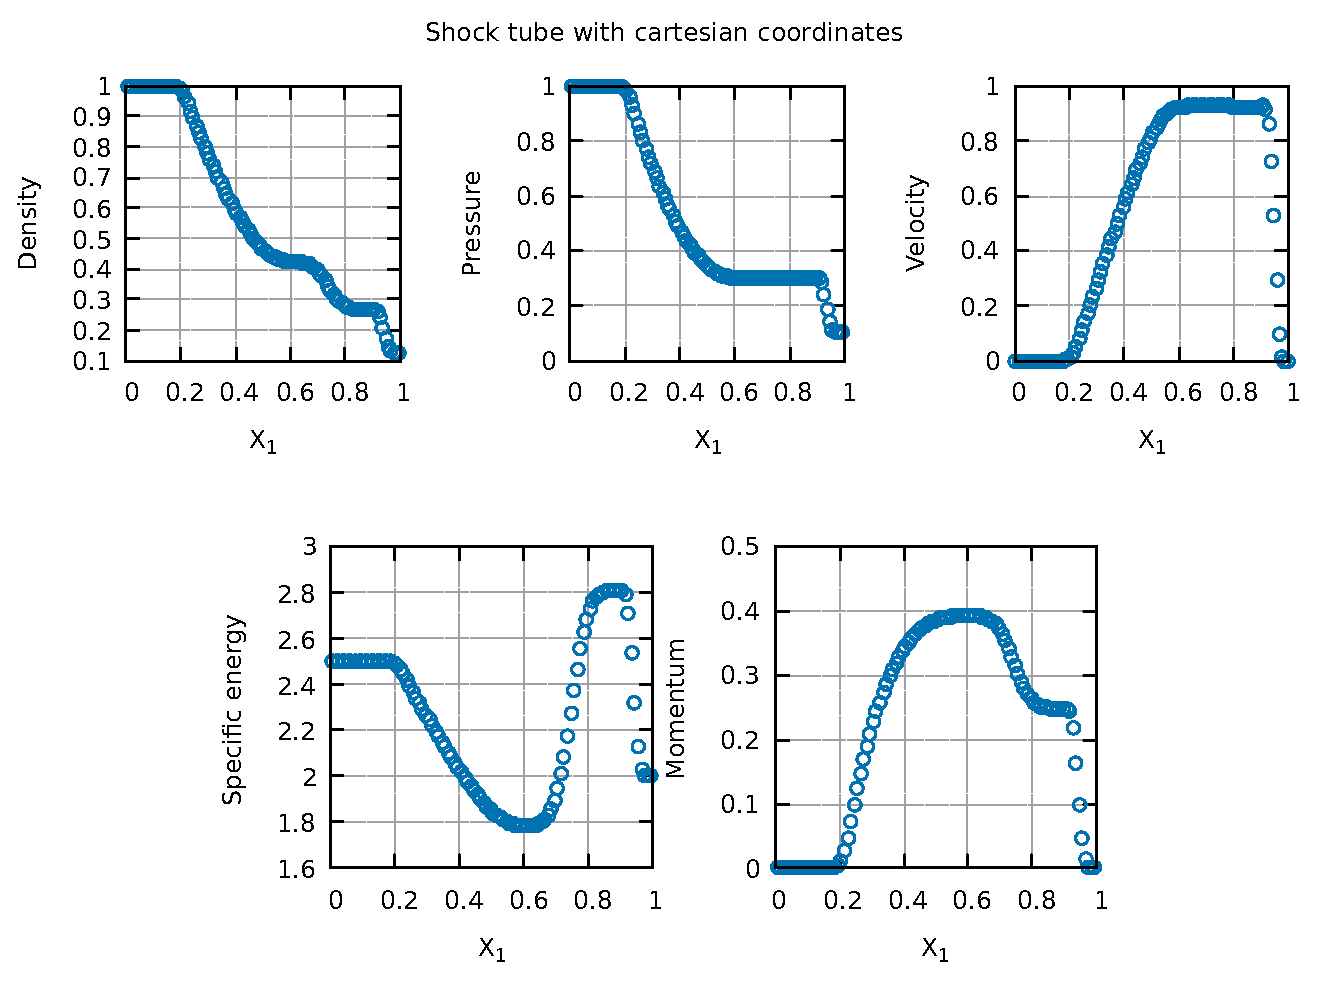
\includegraphics[width=0.9 \linewidth]{cartshock100.pdf}
	\caption{Sod shock tube test for a 100 points grid. From left to right and from top to bottom: $\rho$, $p$, $v$, $\frac{\epsilon}{\rho}$, and $m$ after a $t_{max}=0.245$.}
	\label{fig:cartshock100}
\end{figure}
\begin{figure}[H]
	\centering
	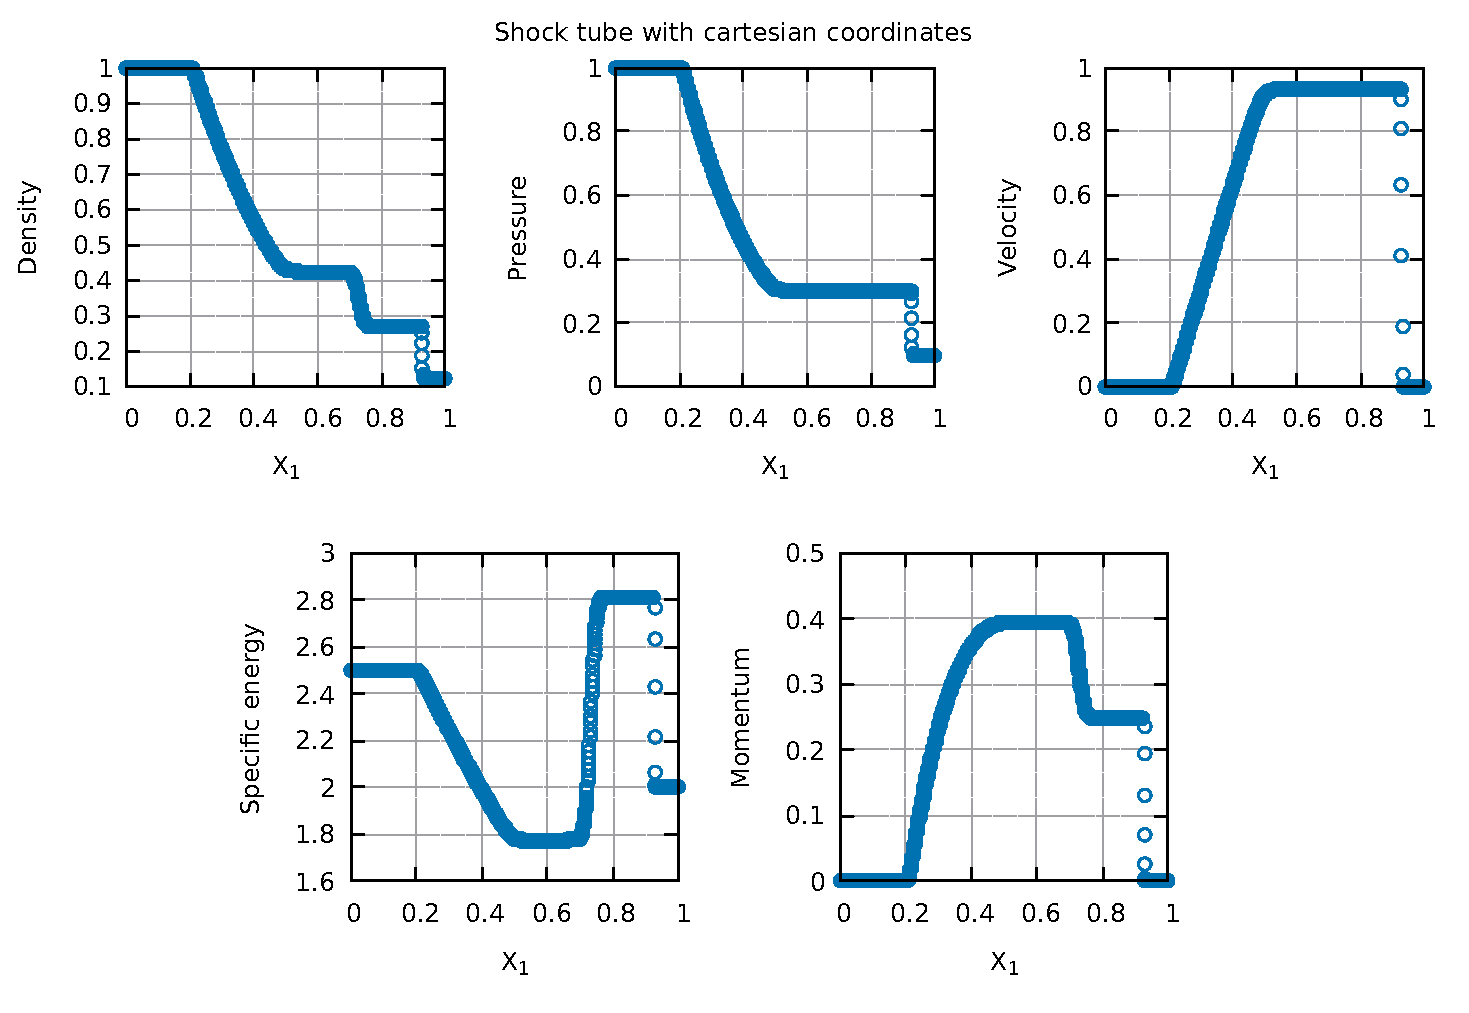
\includegraphics[width=0.9 \linewidth]{cartshock.pdf}
	\caption{Sod shock tube test for a 1000 points grid. From left to right and from top to bottom: $\rho$, $p$, $v$, $\frac{\epsilon}{\rho}$, and $m$ after a $t_{max}=0.245$.}
	\label{fig:cartshock1000}
\end{figure}
\begin{figure}[H]
	\centering
	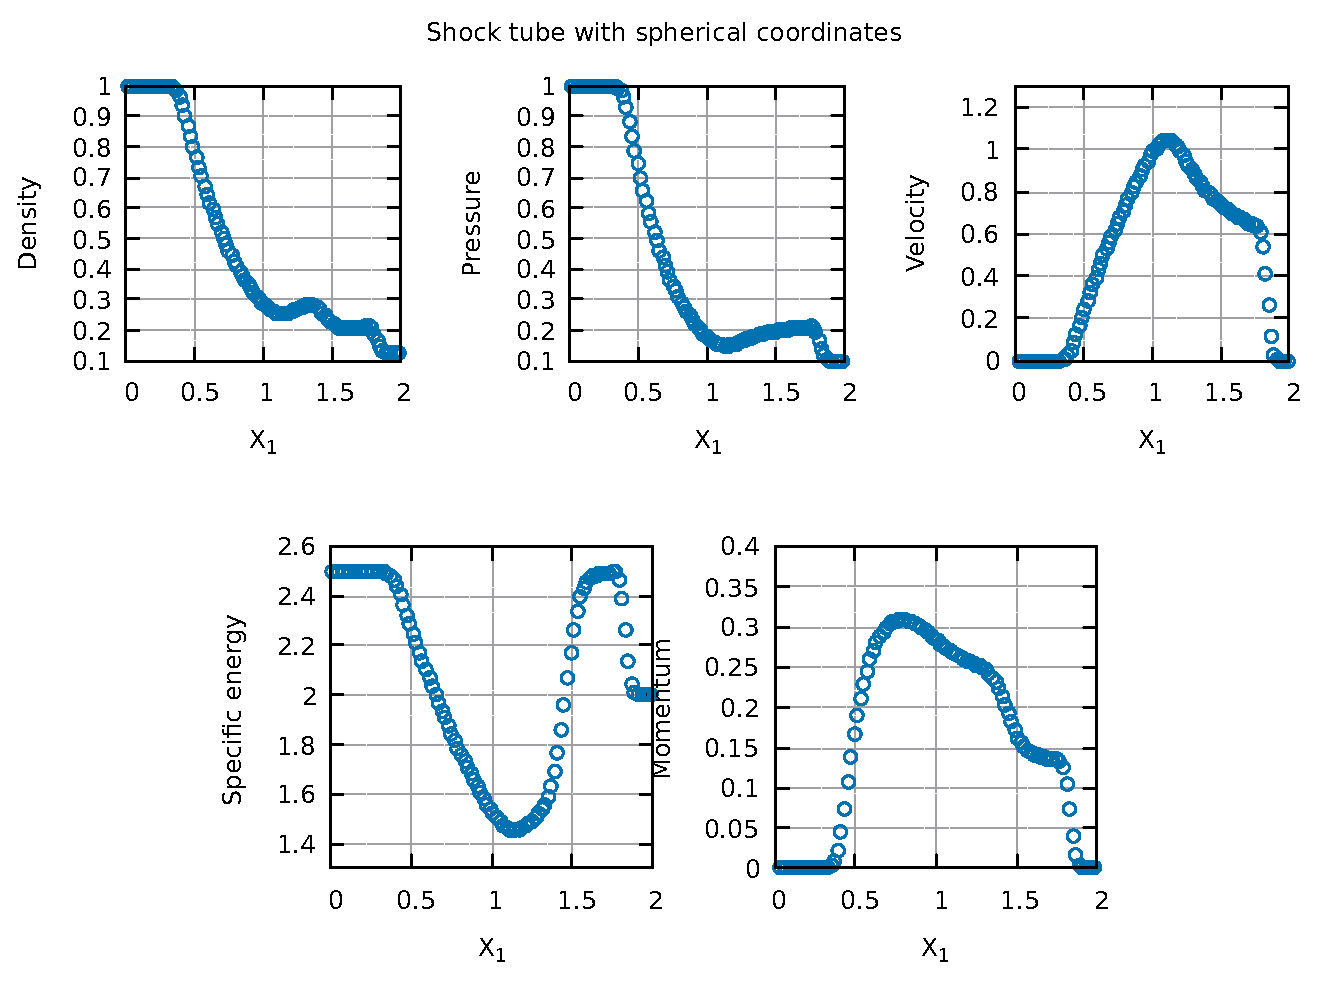
\includegraphics[width=0.9 \linewidth]{spheshock100.pdf}
	\caption{Spherical shock tube test for a 100 points grid. From left to right and from top to bottom: $\rho$, $p$, $v$, $\frac{\epsilon}{\rho}$, and $m$ after a $t_{max}=0.5$.}
	\label{fig:spheshock100}
\end{figure}
\begin{figure}[H]
	\centering
	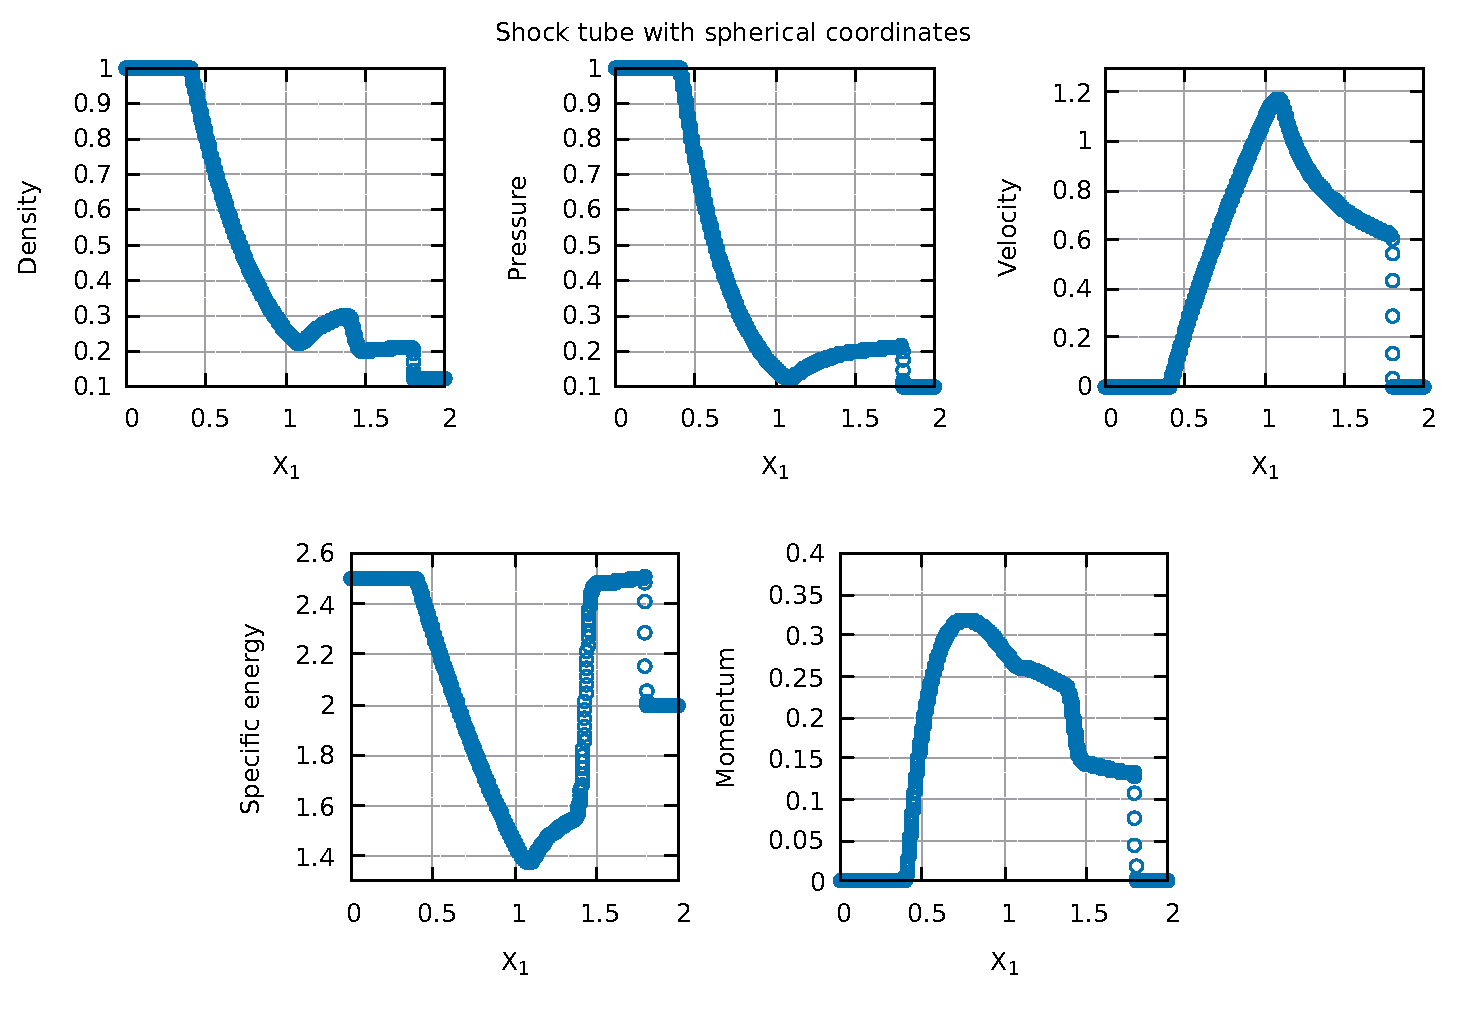
\includegraphics[width=0.9 \linewidth]{spheshock.pdf}
	\caption{Spherical shock tube test for a 1000 points grid. From left to right and from top to bottom: $\rho$, $p$, $v$, $\frac{\epsilon}{\rho}$, and $m$ after a $t_{max}=0.5$.}

	\label{fig:spheshock1000}
\end{figure}
\begin{figure}[H]
	\centering
	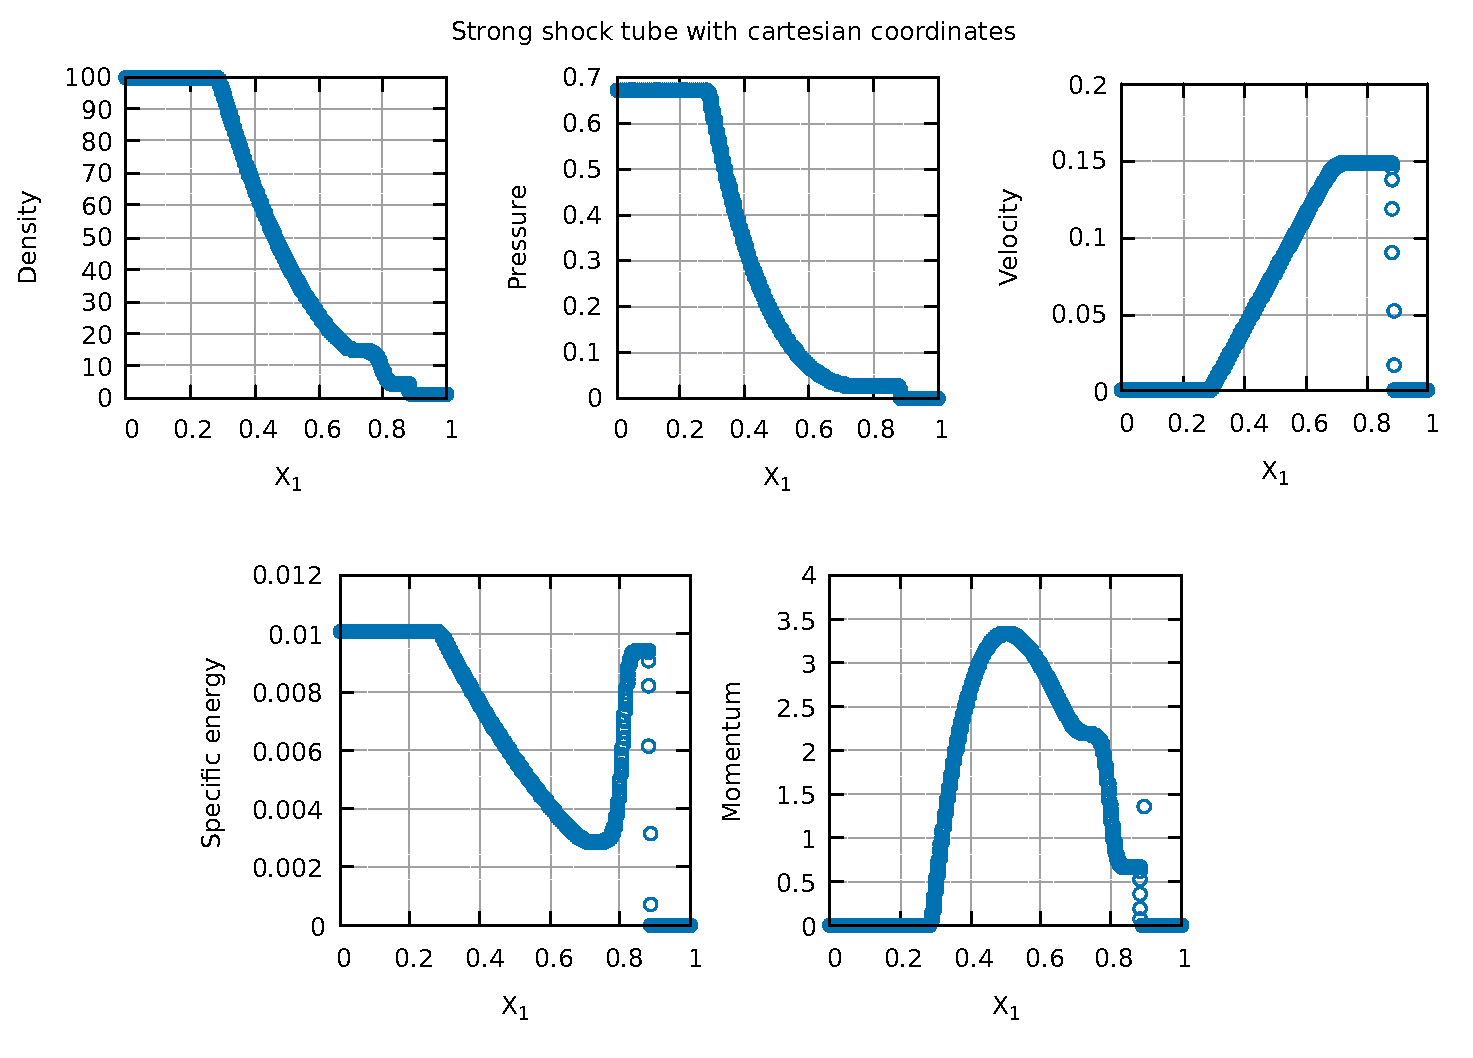
\includegraphics[width=0.9 \linewidth]{strongshocktube.pdf}
	\caption{Strong shock tube test in cartesian coordinates for a 1000 points grid. From left to right and from top to bottom: $\rho$, $p$, $v$, $\frac{\epsilon}{\rho}$, and $m$ after a $t_{max}=2$.}

	\label{fig:strongshock}
\end{figure}
\section{SNR evolution simulation}

\subsection{Physical model}

\subsection{The simulation}

\subsection{Results and discussion}

\section*{Conclusions}

\begin{thebibliography}{5}
	\bibitem{cimatti}
	A. Cimatti, F. Fraternali, and C. Nipoti. Introduction to Galaxy Formation and Evolution.
From Primordial Gas to Present-Day Galaxies. Cambridge University Press, 2020.
	\bibitem{hawley}
	J. F. Hawley, L. L. Smarr, and J. R. Wilson. “A numerical study of nonspherical
black hole accretion. II - Finite differencing and code calibrations”. In: ApJS
55 (1984), pp. 211–246. doi: https://doi.org/10.1086/190953.
\bibitem{omang}
M. Omang, J.K. Trulsen, and S. Børve. “SPH in spherical and cylindrical
coordinates”. In: J. Comput. Phys. 213 (2006), pp. 391–412. doi: https :
//doi.org/10.1016/j.jcp.2005.08.023.
\bibitem{sharma}
P. Sharma, I. J. Parrish, and E. Quataert. “Thermal instability with anisotropic
thermal conduction and adiabatic cosmic rays: implications for cold filaments
in galaxy clusters”. In: ApJ 720 (2010), pp. 652–665. doi: https://doi.org/
10.1088/0004-637X/720/1/652.
\bibitem{stone}
J.M. Stone and M. Norman. “Zeus-2D: A radiation magnetohydrodynamics
code for astrophysical flows in two space dimensions. I. The hydrodynamic
algorithms and tests”. In: ApJS 80(2) (1992), pp. 753–790. doi: https://
doi.org/10.1086/191680.
\end{thebibliography}
\end{document}